%% State Space Modelling of Dynamic Systems
%% Lecture 20: State Feedback Control
\def\FileDate{10/02/02}
\def\FileVersion{1.0}
% ----------------------------------------------------------------
% Notes pages *********************************************************
% ----------------------------------------------------------------

\begin{slide}
   \heading{State Feedback Control}
One of the advantages of state space models is that it is possible to apply state feedback to place the closed loop poles into any desired positions.

\textbf{State Space Design Methodology}

\begin{enumerate}
	\item Design control law to place closed loop poles where desired
	\item If full state not available for feedback, then design an \emph{Observer} to compute the states from the system output
	\item Combine \emph{Observer} and \emph{Controller} -- this takes the place of the \emph{Classical Compensator}
	\item Introduce the \emph{Reference Input} -- affects the closed loop zeros but not the poles making it possible to improve the transient response and tracking accuracy
\end{enumerate}	
\end{slide}


\begin{slide}
   \heading{State Feedback Compensator}
   \begin{center}
   	\resizebox{280pt}{!}{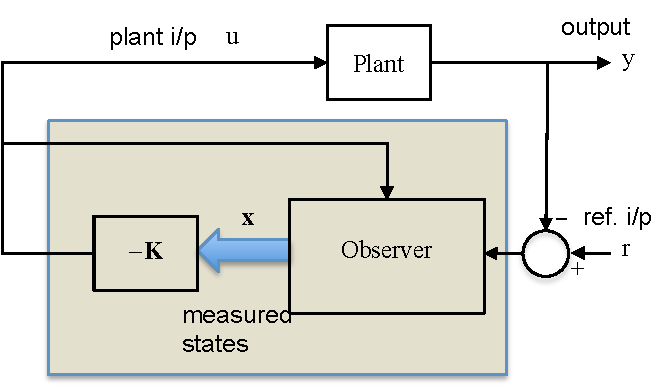
\includegraphics{pictures/statefb.pdf}}
   \end{center}
\end{slide}

\ifslidesonly
\begin{slide}
   \heading{This Lecture}
   \begin{itemize}
   	\item Finding the control law
   	\item State feedback for controller canonical form
   	\item Transfer function model
   	\item Ackermann's formula
   	\item Effect of state feedback on closed-loop zeros
   	\item Effect of plant zeros on the feedback gains
   	\item Pole-selection for good design
   \end{itemize}
\end{slide}
\fi
\section*{Finding the Control Law} % (fold)
\label{sec:finding_the_control_law}

We shall only consider SISO systems here.


\begin{center}
	\resizebox{200pt}{!}{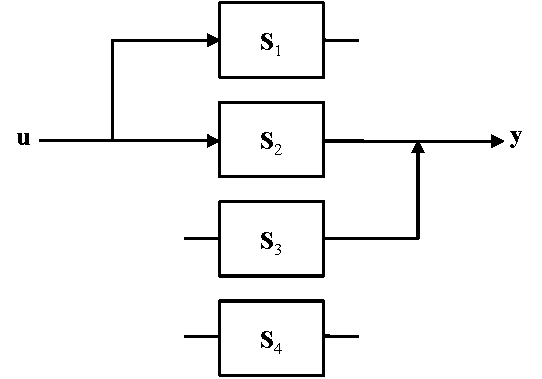
\includegraphics{pictures/partitioning.pdf}}
\end{center}
\endinput

%%% Local Variables: 
%%% mode: latex
%%% TeX-master: "notes"
%%% End:
\ifslidesonly
\begin{slide}
   \heading{Finding the Control Law (1)}
   
\begin{center}
	\resizebox{200pt}{!}{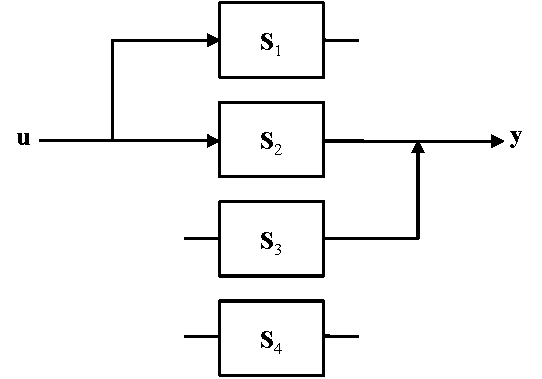
\includegraphics{pictures/partitioning.pdf}}
\end{center}
\endinput

%%% Local Variables: 
%%% mode: latex
%%% TeX-master: "notes"
%%% End:
\end{slide}
\fi

Given the transformation $\mathbf{T}^{-1}\mathbf{AT}=\mathbf{\Lambda}$:
\begin{eqnarray*}
	\mathbf{A}t & = & (\mathbf{T\Lambda T}^{-1}) t \\
	\mathbf{A}^nt^n & = & (\mathbf{T\Lambda T}^{-1})(\mathbf{T\Lambda T}^{-1})\ldots(\mathbf{T\Lambda T}^{-1})t^n \\
	                & = & \mathbf{T\Lambda T}^{-1}\mathbf{T\Lambda T}^{-1}\ldots\mathbf{T\Lambda T}^{-1}t^n \\
	\mathbf{A}^nt^n & = & \mathbf{T\Lambda}\mathbf{I}\mathbf{\Lambda I}\ldots\mathbf{I\Lambda T}^{-1}t^n \\
	\               & = & \mathbf{T\Lambda}^n\mathbf{T}^{-1}t^n \\
\end{eqnarray*}
\endinput

%%% Local Variables: 
%%% mode: latex
%%% TeX-master: "notes"
%%% End:
\ifslidesonly
\begin{slide}
	\heading{Finding the Control Law (2)}
   Given the transformation $\mathbf{T}^{-1}\mathbf{AT}=\mathbf{\Lambda}$:
\begin{eqnarray*}
	\mathbf{A}t & = & (\mathbf{T\Lambda T}^{-1}) t \\
	\mathbf{A}^nt^n & = & (\mathbf{T\Lambda T}^{-1})(\mathbf{T\Lambda T}^{-1})\ldots(\mathbf{T\Lambda T}^{-1})t^n \\
	                & = & \mathbf{T\Lambda T}^{-1}\mathbf{T\Lambda T}^{-1}\ldots\mathbf{T\Lambda T}^{-1}t^n \\
	\mathbf{A}^nt^n & = & \mathbf{T\Lambda}\mathbf{I}\mathbf{\Lambda I}\ldots\mathbf{I\Lambda T}^{-1}t^n \\
	\               & = & \mathbf{T\Lambda}^n\mathbf{T}^{-1}t^n \\
\end{eqnarray*}
\endinput

%%% Local Variables: 
%%% mode: latex
%%% TeX-master: "notes"
%%% End:
\end{slide}
\fi

 
The matrix function becomes:
\begin{eqnarray*}
	f(\mathbf{A}t) & = & f_0\mathbf{TIT}^{-1} + f_1\mathbf{T\Lambda T}^{-1}t + f_2\mathbf{T\Lambda}^2\mathbf{T}^{-1}t^2 + \cdots + f_n\mathbf{T\Lambda}^n\mathbf{T}^{-1}t^n + \cdots \\
	f(\mathbf{A}t) & = & \mathbf{T}\left(f_0\mathbf{I} + f_1\mathbf{\Lambda}t + f_2\mathbf{\Lambda}^2t^2 + \cdots + f_n\mathbf{\Lambda}^nt^n + \cdots \right)\mathbf{T}^{-1}\\
	               & = & \mathbf{T}f(\mathbf{\Lambda}t)\mathbf{T}^{-1}
\end{eqnarray*}
 
The term inside the brackets on the rhs is a diagonal matrix and the $i^\mathrm{th}$ diagonal element is:
\[
f_0+f_1\lambda_it + f_2\lambda_i^2t^2 + \cdots + f_n\lambda_i^nt^ + \cdots
\]
From the Taylor series this must be $f(\lambda_i t)$:
\[
f(\mathbf{A} t)=\mathbf{T} f(\mathbf{\Lambda} t) \mathbf{T}^{-1}
\]   
where $f(\mathbf{\Lambda} t)=\mathrm{diag}\left(f(\lambda_i t)\right)$.

\endinput

%%% Local Variables: 
%%% mode: latex
%%% TeX-master: "notes"
%%% End:
\ifslidesonly
\begin{slide}
	\heading{Finding the Control Law (3)}
   The matrix function becomes:
\begin{eqnarray*}
	f(\mathbf{A}t) & = & f_0\mathbf{TIT}^{-1} + f_1\mathbf{T\Lambda T}^{-1}t + f_2\mathbf{T\Lambda}^2\mathbf{T}^{-1}t^2 + \cdots + f_n\mathbf{T\Lambda}^n\mathbf{T}^{-1}t^n + \cdots \\
	f(\mathbf{A}t) & = & \mathbf{T}\left(f_0\mathbf{I} + f_1\mathbf{\Lambda}t + f_2\mathbf{\Lambda}^2t^2 + \cdots + f_n\mathbf{\Lambda}^nt^n + \cdots \right)\mathbf{T}^{-1}\\
	               & = & \mathbf{T}f(\mathbf{\Lambda}t)\mathbf{T}^{-1}
\end{eqnarray*}
 
The term inside the brackets on the rhs is a diagonal matrix and the $i^\mathrm{th}$ diagonal element is:
\[
f_0+f_1\lambda_it + f_2\lambda_i^2t^2 + \cdots + f_n\lambda_i^nt^ + \cdots
\]
From the Taylor series this must be $f(\lambda_i t)$:
\[
f(\mathbf{A} t)=\mathbf{T} f(\mathbf{\Lambda} t) \mathbf{T}^{-1}
\]   
where $f(\mathbf{\Lambda} t)=\mathrm{diag}\left(f(\lambda_i t)\right)$.

\endinput

%%% Local Variables: 
%%% mode: latex
%%% TeX-master: "notes"
%%% End:
\end{slide}
\fi

The vector $[v_{31}, i_{1}]^T$ is called the ``\emph{state
vector}.'' Its elements are state variables.
\endinput
%%% Local Variables: 
%%% mode: latex
%%% TeX-master: "notes"
%%% End: 

\ifslidesonly
\begin{slide}
	\heading{Finding the Control Law (4)}
   The vector $[v_{31}, i_{1}]^T$ is called the ``\emph{state
vector}.'' Its elements are state variables.
\endinput
%%% Local Variables: 
%%% mode: latex
%%% TeX-master: "notes"
%%% End: 

\end{slide}
\fi



\subsection*{Example 1} % (fold)
\label{sub:example_1}

\textbf{Problem}: Given,
\[
{\bf{\dot x}} = \left[ {\begin{array}{*{20}c}
   { - 4} & 0  \\
   0 & { - 11}  \\
\end{array}} \right]{\bf{x}} + \left[ {\begin{array}{*{20}c}
   1  \\
   { - 1}  \\
\end{array}} \right]u
\]
find the feedback control law which places the closed-loop poles at: $-10\pm j10$.

\textbf{SOLUTION}:
\begin{eqnarray*}
	0 & = & \det \left[ {s{\bf{I}} - {\bf{A}} + {\bf{BK}}} \right] = \det \left\{ {\left. {\left[ {\begin{array}{*{20}c}
	   {s + 4} & 0  \\
	   0 & {s + 11}  \\
	\end{array}} \right] + \left[ {\begin{array}{*{20}c}
	   1  \\
	   { - 1}  \\
	\end{array}} \right]\left[ {\begin{array}{*{20}c}
	   {k_1 } & {k_2 }  \\
	\end{array}} \right]} \right\}} \right. \\
	0 & = & \det \left[ {\begin{array}{*{20}c}
	   {s + 4 + k_1 } & {k_2 }  \\
	   { - k_1 } & {s + 11 - k_2 }  \\
	\end{array}} \right] \\
	0 & = & (s + 4 + k_1 )(s + 11 - k_2 ) - (k_2 )( - k_1 ) \\
	0 & = & (s+4+k_1)(s+11-k_2)+k_1k_2
\end{eqnarray*}
\begin{equation}
	\label{eq:3}
	s^2+(15+k_1-k_2)s+(44+11k_1-4k_2)=0
\end{equation}

Now the desired CE is:
\[
\alpha_c(s)=(s+10-j10)(s+10+j10) = 0
\]
\begin{equation}\label{eq:4}
	s^2+20s+200=0
\end{equation}

Therefore matching coefficients in Eqs. (\ref{eq:3}) and (\ref{eq:4}):
\[
\begin{array}{c}
 s^2 :1 = 1 \to {\rm{OK}} \\ 
 s^1 :15 + k_1  - k_2  = 20 \to k_1  - k_2  = 5 \\ 
 s^0 :44 + 11k_1  - 4k_2  = 200 \to 11k_1  - 4k_2  = 156 \\ 
 \end{array}
\]

 

Solving for the $k$'s:
\[
\left[ {\begin{array}{*{20}c}
   1 & { - 1}  \\
   {11} & { - 4}  \\
\end{array}} \right]\left[ {\begin{array}{*{20}c}
   {k_1 }  \\
   {k_2 }  \\
\end{array}} \right] = \left[ {\begin{array}{*{20}c}
   5  \\
   {156}  \\
\end{array}} \right]
\]
% MathType!MTEF!2!1!+-
% faaagaart1ev2aaaKnaaaaWenf2ys9wBH5garuavP1wzZbqedmvETj
% 2BSbqefm0B1jxALjharqqtubsr4rNCHbGeaGqiVu0Je9sqqrpepC0x
% bbL8FesqqrFfpeea0xe9Lq-Jc9vqaqpepm0xbba9pwe9Q8fs0-yqaq
% pepae9pg0FirpepeKkFr0xfr-xfr-xb9Gqpi0dc9adbaqaaeGaciGa
% aiaabeqaamaabaabaaGcbaWaamWaaeaafaWabeGabaaabaGaam4Aam
% aaBaaaleaacaaIXaaabeaaaOqaaiaadUgadaWgaaWcbaGaaGOmaaqa
% baaaaaGccaGLBbGaayzxaaGaeyypa0ZaaSaaaeaacaaIXaaabaGaey
% OeI0IaaGinaiabgUcaRiaaigdacaaIXaaaamaadmaabaqbamqabiGa
% aaqaaiabgkHiTiaaisdaaeaacaaIXaaabaGaeyOeI0IaaGymaiaaig
% daaeaacaaIXaaaaaGaay5waiaaw2faamaadmaabaqbamqabiqaaaqa
% aiaaiwdaaeaacaaIXaGaaGynaiaaiAdaaaaacaGLBbGaayzxaaGaey
% ypa0ZaaSaaaeaacaaIXaaabaGaaG4naaaadaWadaqaauaadeqaceaa
% aeaacaaIXaGaaG4maiaaiAdaaeaacaaIXaGaaGimaiaaigdaaaaaca
% GLBbGaayzxaaGaeyypa0ZaamWaaeaafaWabeGabaaabaGaaGymaiaa
% iMdacaGGUaGaaGinaiaaiMdacaaIYaGaaGyoaaqaaiaaigdacaaI0a
% GaaiOlaiaaisdacaaIYaGaaGyoaaaaaiaawUfacaGLDbaaaaa!5BC6!
\[
\left[ {\begin{array}{*{20}c}
   {k_1 }  \\
   {k_2 }  \\
\end{array}} \right] = \frac{1}{{ - 4 + 11}}\left[ {\begin{array}{*{20}c}
   { - 4} & 1  \\
   { - 11} & 1  \\
\end{array}} \right]\left[ {\begin{array}{*{20}c}
   5  \\
   {156}  \\
\end{array}} \right] = \frac{1}{7}\left[ {\begin{array}{*{20}c}
   {136}  \\
   {101}  \\
\end{array}} \right] = \left[ {\begin{array}{*{20}c}
   {19.429}  \\
   {14.429}  \\
\end{array}} \right]
\]

 

Therefore the required feedback control law is:
% MathType!MTEF!2!1!+-
% faaagaart1ev2aaaKnaaaaWenf2ys9wBH5garuavP1wzZbqedmvETj
% 2BSbqefm0B1jxALjharqqtubsr4rNCHbGeaGqiVu0Je9sqqrpepC0x
% bbL8FesqqrFfpeea0xe9Lq-Jc9vqaqpepm0xbba9pwe9Q8fs0-yqaq
% pepae9pg0FirpepeKkFr0xfr-xfr-xb9Gqpi0dc9adbaqaaeGaciGa
% aiaabeqaamaabaabaaGcbaGaamyDaiabg2da9iaadkhacqGHsislda
% WadaqaauaadeqabiaaaeaacaaIXaGaaGyoaiaac6cacaaI0aGaaGOm
% aiaaiMdaaeaacaaIXaGaaGinaiaac6cacaaI0aGaaGOmaiaaiMdaaa
% aacaGLBbGaayzxaaGaaCiEaaaa!3DCD!
\[
u = r - \left[ {\begin{array}{*{20}c}
   {19.429} & {14.429}  \\
\end{array}} \right]{\bf{x}}
\]



\textbf{COMMENT}
This matching of coefficients can always be done, though it is tedious for $n>3$, \textbf{EXCEPT} in the case of the \emph{Control Canonical Form}.

% subsection example_1 (end)
 
% section finding_the_control_law (end)

\section*{State Feedback in the Case of the Control Canonical Form} % (fold)
\label{sec:state_feedback_in_the_case_of_the_control_canonical_form}


From previous work the error dynamics are:
\[
\dot{\mathbf{e}} = (\mathbf{A}-\mathbf{LC})\mathbf{e}
\]
Therefore the dynamics of the combined system is:
\[\left[ {\begin{array}{*{20}c}
   {\dot{\mathbf{x}}}  \\
   {\dot{\mathbf{e}}ß}  \\
\end{array}} \right] = \left[ {\begin{array}{*{20}c}
   {\left( {{\bf{A}} - {\bf{BK}}} \right)} & {{\bf{BK}}}  \\
   {\bf{0}} & {\left( {{\bf{A}} - {\bf{LC}}} \right)}  \\
\end{array}} \right]\left[ {\begin{array}{*{20}c}
   {\bf{x}}  \\
   {\bf{e}}  \\
\end{array}} \right] + \left[ {\begin{array}{*{20}c}
   {\bf{B}}  \\
   {\bf{0}}  \\
\end{array}} \right]r
\]
\endinput

%%% Local Variables: 
%%% mode: latex
%%% TeX-master: "notes"
%%% End:
\ifslidesonly
\begin{slide}
	\heading{Control Canonical Form Simplifies Calculation (1)}
   From previous work the error dynamics are:
\[
\dot{\mathbf{e}} = (\mathbf{A}-\mathbf{LC})\mathbf{e}
\]
Therefore the dynamics of the combined system is:
\[\left[ {\begin{array}{*{20}c}
   {\dot{\mathbf{x}}}  \\
   {\dot{\mathbf{e}}ß}  \\
\end{array}} \right] = \left[ {\begin{array}{*{20}c}
   {\left( {{\bf{A}} - {\bf{BK}}} \right)} & {{\bf{BK}}}  \\
   {\bf{0}} & {\left( {{\bf{A}} - {\bf{LC}}} \right)}  \\
\end{array}} \right]\left[ {\begin{array}{*{20}c}
   {\bf{x}}  \\
   {\bf{e}}  \\
\end{array}} \right] + \left[ {\begin{array}{*{20}c}
   {\bf{B}}  \\
   {\bf{0}}  \\
\end{array}} \right]r
\]
\endinput

%%% Local Variables: 
%%% mode: latex
%%% TeX-master: "notes"
%%% End:
\end{slide}
\fi


When the initial conditions of the state-variables are all zero,
this reduces to the transfer matrix model
\begin{equation}\label{eqn:transfer-function}
  \mathbf{Y}=\left[\mathbf{C}\left[s\mathbf{I}-\mathbf{A}\right]^{-1}\mathbf{B}+\mathbf{D}\right]\mathbf{U}
\end{equation}

\endinput

%%% Local Variables: 
%%% mode: latex
%%% TeX-master: "notes"
%%% End: 

When the observer canonical form is not used, then the design of the observer is more difficult. Ackermann's formula can be adapted as follows:
% MathType!MTEF!2!1!+-
% faaagaart1ev2aaaKnaaaaWenf2ys9wBH5garuavP1wzZbqedmvETj
% 2BSbqefm0B1jxALjharqqtubsr4rNCHbGeaGqiVu0Je9sqqrpepC0x
% bbL8FesqqrFfpeea0xe9Lq-Jc9vqaqpepm0xbba9pwe9Q8fs0-yqaq
% pepae9pg0FirpepeKkFr0xfr-xfr-xb9Gqpi0dc9adbaqaaeGaciGa
% aiaabeqaamaabaabaaGcbaGaaCitamaaCaaaleqabaGaamivaaaaki
% abg2da9maadmaabaqbamqabeabaaaabaGaaGimaaqaaiablAcilbqa
% aiaaicdaaeaacaaIXaaaaaGaay5waiaaw2faaiaad+eadaahaaWcbe
% qaaiabgkHiTiaaigdaaaGccqaHXoqydaWgaaWcbaGaam4yaaqabaGc
% caGGOaGaaCyqamaaCaaaleqabaGaamivaaaakiaacMcaaaa!3EF6!
\[
{\bf{L}}^T  = \left[ {\begin{array}{*{20}c}
   0 &  \ldots  & 0 & 1  \\
\end{array}} \right]\mathcal{O}^{ - 1} \alpha _e ({\bf{A}}^T )
\]
$\mathcal{O}$ is the observability matrix:
\[
\mathcal{O}=[\mathbf{C}^T\vdots\mathbf{A}^T\mathbf{C}^T\vdots\cdots\vdots(\mathbf{A}^T)^{n-1}\mathbf{C}^T]
\]
and if $\alpha_e(s)=s^n + \alpha_1s^{n-1}+\cdots+\alpha_n$ then \[\alpha_e(\mathbf{A}^T)=(\mathbf{A}^T)^n + \alpha_1(\mathbf{A}^T)^{n-1}+\cdots+\mathbf{I}\alpha_n.\]
 

Notice that if the system is unobservable, then the matrix inverse $\mathcal{O}^{-1}$ does not exist and we cannot design an observer for this system.


 
 

\endinput

%%% Local Variables: 
%%% mode: latex
%%% TeX-master: "notes"
%%% End:
\ifslidesonly
\begin{slide}
	\heading{Control Canonical Form (2)}
   When the initial conditions of the state-variables are all zero,
this reduces to the transfer matrix model
\begin{equation}\label{eqn:transfer-function}
  \mathbf{Y}=\left[\mathbf{C}\left[s\mathbf{I}-\mathbf{A}\right]^{-1}\mathbf{B}+\mathbf{D}\right]\mathbf{U}
\end{equation}

\endinput

%%% Local Variables: 
%%% mode: latex
%%% TeX-master: "notes"
%%% End: 

\end{slide}
\begin{slide}
	\heading{Control Canonical Form (3)}
   When the observer canonical form is not used, then the design of the observer is more difficult. Ackermann's formula can be adapted as follows:
% MathType!MTEF!2!1!+-
% faaagaart1ev2aaaKnaaaaWenf2ys9wBH5garuavP1wzZbqedmvETj
% 2BSbqefm0B1jxALjharqqtubsr4rNCHbGeaGqiVu0Je9sqqrpepC0x
% bbL8FesqqrFfpeea0xe9Lq-Jc9vqaqpepm0xbba9pwe9Q8fs0-yqaq
% pepae9pg0FirpepeKkFr0xfr-xfr-xb9Gqpi0dc9adbaqaaeGaciGa
% aiaabeqaamaabaabaaGcbaGaaCitamaaCaaaleqabaGaamivaaaaki
% abg2da9maadmaabaqbamqabeabaaaabaGaaGimaaqaaiablAcilbqa
% aiaaicdaaeaacaaIXaaaaaGaay5waiaaw2faaiaad+eadaahaaWcbe
% qaaiabgkHiTiaaigdaaaGccqaHXoqydaWgaaWcbaGaam4yaaqabaGc
% caGGOaGaaCyqamaaCaaaleqabaGaamivaaaakiaacMcaaaa!3EF6!
\[
{\bf{L}}^T  = \left[ {\begin{array}{*{20}c}
   0 &  \ldots  & 0 & 1  \\
\end{array}} \right]\mathcal{O}^{ - 1} \alpha _e ({\bf{A}}^T )
\]
$\mathcal{O}$ is the observability matrix:
\[
\mathcal{O}=[\mathbf{C}^T\vdots\mathbf{A}^T\mathbf{C}^T\vdots\cdots\vdots(\mathbf{A}^T)^{n-1}\mathbf{C}^T]
\]
and if $\alpha_e(s)=s^n + \alpha_1s^{n-1}+\cdots+\alpha_n$ then \[\alpha_e(\mathbf{A}^T)=(\mathbf{A}^T)^n + \alpha_1(\mathbf{A}^T)^{n-1}+\cdots+\mathbf{I}\alpha_n.\]
 

Notice that if the system is unobservable, then the matrix inverse $\mathcal{O}^{-1}$ does not exist and we cannot design an observer for this system.


 
 

\endinput

%%% Local Variables: 
%%% mode: latex
%%% TeX-master: "notes"
%%% End:
\end{slide}
\fi


 
\begin{itemize}
	\item Rule of thumb: observer poles can be faster than the controller poles (i.e. further from the origin) by a factor of 2 to 6. This makes the effect of the observer dynamics short-term and the overall response is dominated by the controller poles.
	\item If noise/disturbance is present this has an effect on the choice:
	\begin{description}
		\item[Process noise $w$:] $d\mathbf{x}/dt=\mathbf{Ax}+\mathbf{B}u+\mathbf{B}_1 w$
		\item[Sensor noise $v$:]  $y = \mathbf{C}x+v$
		\item[Observer:] $d\hat{\mathbf{x}}=\mathbf{A}\hat{\mathbf{x}}+\mathbf{B}u+\mathbf{L}(y-\mathbf{C}\hat{\mathbf{x}})$
		\item[Error $\mathbf{e}=\mathbf{x}-\hat{\mathbf{x}}$:] $d\mathbf{e}/dt=(\mathbf{A}-\mathbf{LC})\mathbf{e}+\mathbf{B}_1 w - \mathbf{L}v.$
	\end{description}
\end{itemize}

\endinput

%%% Local Variables: 
%%% mode: latex
%%% TeX-master: "notes"
%%% End:
\ifslidesonly
\begin{slide}
	\heading{Control Canonical Form (4)}
   \begin{itemize}
	\item Rule of thumb: observer poles can be faster than the controller poles (i.e. further from the origin) by a factor of 2 to 6. This makes the effect of the observer dynamics short-term and the overall response is dominated by the controller poles.
	\item If noise/disturbance is present this has an effect on the choice:
	\begin{description}
		\item[Process noise $w$:] $d\mathbf{x}/dt=\mathbf{Ax}+\mathbf{B}u+\mathbf{B}_1 w$
		\item[Sensor noise $v$:]  $y = \mathbf{C}x+v$
		\item[Observer:] $d\hat{\mathbf{x}}=\mathbf{A}\hat{\mathbf{x}}+\mathbf{B}u+\mathbf{L}(y-\mathbf{C}\hat{\mathbf{x}})$
		\item[Error $\mathbf{e}=\mathbf{x}-\hat{\mathbf{x}}$:] $d\mathbf{e}/dt=(\mathbf{A}-\mathbf{LC})\mathbf{e}+\mathbf{B}_1 w - \mathbf{L}v.$
	\end{description}
\end{itemize}

\endinput

%%% Local Variables: 
%%% mode: latex
%%% TeX-master: "notes"
%%% End:
\end{slide}
\fi

 
\subsection*{Example 2} % (fold)
\label{sub:example_2}

\textbf{Problem}: Given the system TF:
\[
G(s) = \frac{7}{(s+4)(s+11)}
\]
find the control law for the control canonical form which places the closed loop poles at $s=−10\pm j10$.

\textbf{SOLUTION}:
\[
G(s) = \frac{7}{(s+4)(s+11)} = \frac{7}{(s^2+15s+44)}
\]
 
The control canonical form has matrices:
\[
{\bf{A}} = \left[ {\begin{array}{*{20}c}
   { - 15} & { - 44}  \\
   1 & 0  \\
\end{array}} \right];\quad {\bf{B}} = \left[ {\begin{array}{*{20}c}
   1  \\
   0  \\
\end{array}} \right];\quad {\bf{C}} = \left[ {\begin{array}{*{20}c}
   0 & 7  \\
\end{array}} \right];\quad {\bf{D}} = 0
\]
 
\textbf{NB}:  $\mathbf{C}$ is obtained from the TF numerator $(0s+7)$.
so:    
\[
{\bf{A}} - {\bf{BK}} = \left[ {\begin{array}{*{20}c}
   { - 15 - k_1 } & { - 44 - k_2 }  \\
   1 & 0  \\
\end{array}} \right]
\]
and the closed loop CE is:
\begin{equation}
	s^2+(15+k_1)s+(44+k_2)=0 \label{eq:7}
\end{equation}
The desired CE is:
\[
\alpha_c(s)=(s+10-j10)(s+10+j10) = 0
\]
\begin{equation}\label{eq:8}
	s^2+20s+200=0
\end{equation}
 
Comparing Eqs. (\ref{eq:7})  and  (\ref{eq:8}) gives:
% MathType!MTEF!2!1!+-
% faaagaart1ev2aaaKnaaaaWenf2ys9wBH5garuavP1wzZbqedmvETj
% 2BSbqefm0B1jxALjharqqtubsr4rNCHbGeaGqiVu0Je9sqqrpepC0x
% bbL8FesqqrFfpeea0xe9Lq-Jc9vqaqpepm0xbba9pwe9Q8fs0-yqaq
% pepae9pg0FirpepeKkFr0xfr-xfr-xb9Gqpi0dc9adbaqaaeGaciGa
% aiaabeqaamaabaabaaGcbaGaaGymaiaaiwdacqGHRaWkcaWGRbWaaS
% baaSqaaiaaigdaaeqaaOGaeyypa0JaaGOmaiaaicdacqGHsgIRcaWG
% RbWaaSbaaSqaaiaaigdaaeqaaOGaeyypa0JaaGynaaaa!3A5E!
\[
15 + k_1  = 20 \to k_1  = 5
\]
and
% MathType!MTEF!2!1!+-
% faaagaart1ev2aaaKnaaaaWenf2ys9wBH5garuavP1wzZbqedmvETj
% 2BSbqefm0B1jxALjharqqtubsr4rNCHbGeaGqiVu0Je9sqqrpepC0x
% bbL8FesqqrFfpeea0xe9Lq-Jc9vqaqpepm0xbba9pwe9Q8fs0-yqaq
% pepae9pg0FirpepeKkFr0xfr-xfr-xb9Gqpi0dc9adbaqaaeGaciGa
% aiaabeqaamaabaabaaGcbaGaaGymaiaaiwdacqGHRaWkcaWGRbWaaS
% baaSqaaiaaigdaaeqaaOGaeyypa0JaaGOmaiaaicdacqGHsgIRcaWG
% RbWaaSbaaSqaaiaaigdaaeqaaOGaeyypa0JaaGynaaaa!3A5E!
\[
44 + k_2  = 200 \to k_2  = 156
\]
giving the control law as:   
\[
u = r - \left[ {\begin{array}{*{20}c}
   {5} & {156}  \\
\end{array}} \right]{\bf{x}}
\]

% subsection example_2 (end)Given the system TF:


% section state_feedback_in_the_case_of_the_control_canonical_form (end)

\section*{A Transfer Function Model of State Feedback} % (fold)
\label{sec:a_transfer_function_model_of_state_feedback}

The last example had a system TF with no zeros. In this case it is easy to construct the equivalent classical controller. We had the feedback law:
\[
u=r-5x_1-156x_2
\]

Now $y=7x_2$ and $\dot{x}_2=x_1$ therefore $X_2(s)=Y(s)/7$ and $X_1(s)=sX_2(s)=sY(s)/7$. Therefore
\begin{eqnarray*}
	U(s) & = & R(s)-rX_1(s)-156X_2(s) \\
	& = & R(s) - \frac{1}{7}(5s+156)Y(s)
\end{eqnarray*}

\endinput

%%% Local Variables: 
%%% mode: latex
%%% TeX-master: "notes"
%%% End:
\ifslidesonly
\begin{slide}
	\heading{Transfer Function Model of State Feedback (1)}
   The last example had a system TF with no zeros. In this case it is easy to construct the equivalent classical controller. We had the feedback law:
\[
u=r-5x_1-156x_2
\]

Now $y=7x_2$ and $\dot{x}_2=x_1$ therefore $X_2(s)=Y(s)/7$ and $X_1(s)=sX_2(s)=sY(s)/7$. Therefore
\begin{eqnarray*}
	U(s) & = & R(s)-rX_1(s)-156X_2(s) \\
	& = & R(s) - \frac{1}{7}(5s+156)Y(s)
\end{eqnarray*}

\endinput

%%% Local Variables: 
%%% mode: latex
%%% TeX-master: "notes"
%%% End:
\end{slide}
\fi

\[
s{\bf{\hat X}}(s) =  {\bf{A\hat X}}(s) + {\bf{B}}U(s) + {\bf{L}}\left( {Y(s) - {\bf{C\hat X}}}(s) \right)
\]
then,
\[
\left( {s{\bf{I}} - {\bf{A}} + {\bf{LC}}} \right){\bf{\hat X}}(s) = {\bf{B}}U(s) + {\bf{L}}Y(s) 
\]
or,
\[
{\bf{\hat X}}(s) = {\bf{M}}^{ - 1} {\bf{B}}U(s) + {\bf{M}}^{ - 1} {\bf{L}}Y(s)
\]


\endinput

%%% Local Variables: 
%%% mode: latex
%%% TeX-master: "notes"
%%% End:
\ifslidesonly
\begin{slide}
	\heading{Transfer Function Model of State Feedback (2)}
   \[
s{\bf{\hat X}}(s) =  {\bf{A\hat X}}(s) + {\bf{B}}U(s) + {\bf{L}}\left( {Y(s) - {\bf{C\hat X}}}(s) \right)
\]
then,
\[
\left( {s{\bf{I}} - {\bf{A}} + {\bf{LC}}} \right){\bf{\hat X}}(s) = {\bf{B}}U(s) + {\bf{L}}Y(s) 
\]
or,
\[
{\bf{\hat X}}(s) = {\bf{M}}^{ - 1} {\bf{B}}U(s) + {\bf{M}}^{ - 1} {\bf{L}}Y(s)
\]


\endinput

%%% Local Variables: 
%%% mode: latex
%%% TeX-master: "notes"
%%% End:
\end{slide}
\fi



% section a_transfer_function_model_of_state_feedback (end)

\section*{Ackermann's Formula} % (fold)
\label{sec:ackermann_s_formula}

\subsection*{State Feedback Design for any Form of State Space Model} % (fold)
As stated previously, the derivation of the feedback law is tedious for systems of order  $n>3$  except in the case of the controller canonical form. One approach to the problem is to transform the given model to controller canonical form, derive the control law in terms of these states and then transform back to the original system. Ackermann derived the following formula by this method.
\ifslidesonly
\begin{slide}
   \heading{State Feedback Design for any Form of State Space Model}
\begin{itemize}
	\item As stated previously, the derivation of the feedback law is tedious for systems of order  $n>3$  except in the case of the controller canonical form.
	\item One approach to the problem is to transform the given model to controller canonical form, derive the control law in terms of these states and then transform back to the original system.
	\item Ackermann derived the following formula by this method.
\end{itemize}
\end{slide}
\fi

\subsection*{The formula} % (fold)
\label{sub:the_formula}

Now
\[
U(s) =  - {\bf{K\hat X}}(s) 
\]
so
\[
U (s) =   - {\bf{K}}\left( {{\bf{M}}^{ - 1} {\bf{B}}U(s) + {\bf{M}}^{ - 1} {\bf{L}}Y(s)} \right) 
\]
\[
 \left( {1 + {\bf{KM}}^{ - 1} {\bf{B}}} \right)U(s) =  - {\bf{KM}}^{ - 1} {\bf{L}}Y(s)
\]

\[ 
H\left( s \right) =  - \frac{U(s)}{Y(sßß)} = \frac{{{\bf{KM}}^{ - 1} {\bf{L}}}}{{1 + {\bf{KM}}^{ - 1} {\bf{B}}}} 
\]




\endinput

%%% Local Variables: 
%%% mode: latex
%%% TeX-master: "notes"
%%% End:
\ifslidesonly
\begin{slide}
	\heading{Ackermann's Formula}
   Now
\[
U(s) =  - {\bf{K\hat X}}(s) 
\]
so
\[
U (s) =   - {\bf{K}}\left( {{\bf{M}}^{ - 1} {\bf{B}}U(s) + {\bf{M}}^{ - 1} {\bf{L}}Y(s)} \right) 
\]
\[
 \left( {1 + {\bf{KM}}^{ - 1} {\bf{B}}} \right)U(s) =  - {\bf{KM}}^{ - 1} {\bf{L}}Y(s)
\]

\[ 
H\left( s \right) =  - \frac{U(s)}{Y(sßß)} = \frac{{{\bf{KM}}^{ - 1} {\bf{L}}}}{{1 + {\bf{KM}}^{ - 1} {\bf{B}}}} 
\]




\endinput

%%% Local Variables: 
%%% mode: latex
%%% TeX-master: "notes"
%%% End:
\end{slide}
\fi

$\mathcal{C}$ is the controllability matrix (see Lecture 19):
\[
\mathcal{C} = [\mathbf{B}\vdots\mathbf{AB}\vdots\cdots\vdots\mathbf{A}^{n-1}\mathbf{B}]
\]
and
\[
\alpha_c(\mathbf{A})=\mathbf{A}^n + \alpha_1\mathbf{A}^{n-1}+ \cdots + \alpha_n\mathbf{I}
\]

\endinput

%%% Local Variables: 
%%% mode: latex
%%% TeX-master: "notes"
%%% End:
\ifslidesonly
\begin{slide}
	\heading{Explanation of the Terms}
   $\mathcal{C}$ is the controllability matrix (see Lecture 19):
\[
\mathcal{C} = [\mathbf{B}\vdots\mathbf{AB}\vdots\cdots\vdots\mathbf{A}^{n-1}\mathbf{B}]
\]
and
\[
\alpha_c(\mathbf{A})=\mathbf{A}^n + \alpha_1\mathbf{A}^{n-1}+ \cdots + \alpha_n\mathbf{I}
\]

\endinput

%%% Local Variables: 
%%% mode: latex
%%% TeX-master: "notes"
%%% End:
\end{slide}
\fi

\[
u = r - \mathbf{K}\hat{\mathbf{x}}
\]
Taking Laplace transforms
\[
U = R - \mathbf{K}\hat{\mathbf{X}}
\]

\endinput

%%% Local Variables: 
%%% mode: latex
%%% TeX-master: "notes"
%%% End:
\ifslidesonly
\begin{slide}
	\heading{Caveats}
   \[
u = r - \mathbf{K}\hat{\mathbf{x}}
\]
Taking Laplace transforms
\[
U = R - \mathbf{K}\hat{\mathbf{X}}
\]

\endinput

%%% Local Variables: 
%%% mode: latex
%%% TeX-master: "notes"
%%% End:
\end{slide}
\fi

\subsection*{Matlab Function}
\[
U=R-\mathbf{K}\left(\mathbf{M}^{-1}\mathbf{B}U + \mathbf{M}^{-1}{\bf{L}}Y\right)
\]
Re-arranging:
\[
\left(\mathbf{KM}^{-1}\mathbf{B}+1\right)U=R-\mathbf{KM}^{-1}\mathbf{L}Y
\]
therefore,
\[
U=\frac{1}{\mathbf{KM}^{-1}\mathbf{B}+1}R-\frac{\mathbf{KM}^{-1}\mathbf{L}}{\mathbf{KM}^{-1}\mathbf{B}+1}Y
\]

\endinput

%%% Local Variables: 
%%% mode: latex
%%% TeX-master: "notes"
%%% End:
\ifslidesonly
\begin{slide}
	\heading{Matlab Function}
   \[
U=R-\mathbf{K}\left(\mathbf{M}^{-1}\mathbf{B}U + \mathbf{M}^{-1}{\bf{L}}Y\right)
\]
Re-arranging:
\[
\left(\mathbf{KM}^{-1}\mathbf{B}+1\right)U=R-\mathbf{KM}^{-1}\mathbf{L}Y
\]
therefore,
\[
U=\frac{1}{\mathbf{KM}^{-1}\mathbf{B}+1}R-\frac{\mathbf{KM}^{-1}\mathbf{L}}{\mathbf{KM}^{-1}\mathbf{B}+1}Y
\]

\endinput

%%% Local Variables: 
%%% mode: latex
%%% TeX-master: "notes"
%%% End:
\end{slide}
\fi

% subsection the_formula (end)
 
\subsection*{Example 3} % (fold)
\label{ssec:example_2}

\textbf{Problem}: 
Given:
\[
{\bf{A}} = \left[ {\begin{array}{*{20}c}
   1 & 2  \\
   { - 1} & 1  \\
\end{array}} \right]\quad {\rm{and}}\quad {\bf{B}} = \left[ {\begin{array}{*{20}c}
   1  \\
   { - 2}  \\
\end{array}} \right]
\]
find the feedback vector $\mathbf{K}$ to place the closed loop poles at $s = −1,\ −1$ using Ackermann's formula.

\textbf{SOLUTION}:
\[
\alpha_c(s) = (s + 1)(s + 1) = s^2 + 2s + 1
\]
therefore
\[
\alpha_c(s) = \mathbf{A}s^2 + 2\mathbf{A}s + \mathbf{I}
\]
\[
\alpha _c ({\bf{A}}) = \left[ {\begin{array}{*{20}c}
   { - 1} & 4  \\
   { - 2} & { - 1}  \\
\end{array}} \right] + 2\left[ {\begin{array}{*{20}c}
   1 & 2  \\
   { - 1} & 1  \\
\end{array}} \right] + \left[ {\begin{array}{*{20}c}
   1 & 0  \\
   0 & 1  \\
\end{array}} \right] = \left[ {\begin{array}{*{20}c}
   2 & 8  \\
   { - 4} & 2  \\
\end{array}} \right]
\]

\[
{\bf{AB}} = \left[ {\begin{array}{*{20}c}
   { - 3}  \\
   { - 3}  \\
\end{array}} \right];\quad \mathcal{C} = \left[ {{\bf{A}} \vdots {\bf{AB}}} \right] = \left[ {\begin{array}{*{20}c}
   1 & { - 3}  \\
   { - 2} & { - 3}  \\
\end{array}} \right]
\]

\begin{eqnarray*}
	{\bf{K}} & = & \left[ {\begin{array}{*{20}c}
	   0 &  \cdots  & 0 & 1  \\
	\end{array}} \right]\mathcal{C}^{ - 1} \alpha _c ({\bf{A}}) \\
	& = & \left[ {\begin{array}{*{20}c}
	   0 & 1  \\
	\end{array}} \right]\left[ {\begin{array}{*{20}c}
	   1 & { - 3}  \\
	   { - 2} & { - 3}  \\
	\end{array}} \right]^{ - 1} \left[ {\begin{array}{*{20}c}
	   2 & 8  \\
	   { - 4} & 2  \\
	\end{array}} \right] \\
	& = & \left[ {\begin{array}{*{20}c}
	   0 & 1  \\
	\end{array}} \right]\frac{\left[ {\begin{array}{*{20}c}
	   { -3 } & { 3 }  \\
	   { 2 } & { 1 }  \\
	\end{array}} \right]}{-3-(+6)} \left[ {\begin{array}{*{20}c}
	   2 & 8  \\
	   { - 4} & 2  \\
	\end{array}} \right] \\
	& = & \left[ {\begin{array}{*{20}c}
	   0 & 1  \\
	\end{array}} \right]\frac{1}{-9}\left[ \begin{array}{*{20}c}
	   { -18 } & { -18 }  \\
	   { 0 } & { 18 }  \\
	\end{array} \right] \\
	& = & \left[ {\begin{array}{*{20}c}
	   0 & 1  \\
	\end{array}} \right]\left[ \begin{array}{*{20}c}
	   { 2 } & { 2 }  \\
	   { 0 } & { -2 }  \\
	\end{array} \right] \\
	& = & \left[ {\begin{array}{*{20}c}
	   0 & -2  \\
	\end{array}} \right]
\end{eqnarray*}
% subsection example_3 (end)

\subsection*{Solution in Matlab} % (fold)
\label{sub:solution_in_matlab}
\begin{verbatim}
% Using the formula
A = [1 2; -1 1]; B = [1; -2];
alpha_c = A * A + 2 * A + eye(2);
K = [0 1] * inv(ctrb(A, B)) * alpha_c

% Using the function Acker
P = [-1, -1] % vector of desired pole locations
Ka = acker(A, B, P)
\end{verbatim}
\ifslidesonly
\begin{slide}
   \heading{Solution in Matlab(1)}
\begin{verbatim}
A = [1 2; -1 1]; B = [1; -2];
alpha_c = A * A + 2 * A + eye(2);
K = [0 1] * inv(ctrb(A, B)) * alpha_c
\end{verbatim}
\end{slide}
\begin{slide}
   \heading{Solution in Matlab(2)}
\begin{verbatim}
% Using the function Acker
P = [-1, -1] % vector of desired pole locations
Ka = acker(A, B, P)
\end{verbatim}
\end{slide}
\fi 
% subsection solution_in_matlab (end)


 


 

% section ackermann_s_formula (end)

\section*{Effect of State Feedback on the Closed Loop Zeros} % (fold)
\label{sec:effect_of_state_feedback_on_the_closed_loop_zeros}

Since,
\[
u = r - \mathbf{Kx}
\]
then the closed-loop system is:
\begin{eqnarray*}
	\dot{\mathbf{x}} & = & \mathbf{A}\mathbf{x}+\mathbf{B}u;\ y = \mathbf{C}\mathbf{x}+\mathbf{D}u \\
	\dot{\mathbf{x}} & = & \mathbf{A}\mathbf{x}+\mathbf{B}(r - \mathbf{K}\mathbf{x});\ y = \mathbf{C}\mathbf{x}+\mathbf{D}(r - \mathbf{K}\mathbf{x}) \\
	\dot{\mathbf{x}} & = & (\mathbf{A}-\mathbf{B}\mathbf{K})\mathbf{x}+\mathbf{B}r;\ y = (\mathbf{C}-\mathbf{D}\mathbf{K})\mathbf{x}+\mathbf{D}r \\
\end{eqnarray*}

\endinput

%%% Local Variables: 
%%% mode: latex
%%% TeX-master: "notes"
%%% End:
\ifslidesonly
\begin{slide}
	\heading{Closed-Loop System}
   Since,
\[
u = r - \mathbf{Kx}
\]
then the closed-loop system is:
\begin{eqnarray*}
	\dot{\mathbf{x}} & = & \mathbf{A}\mathbf{x}+\mathbf{B}u;\ y = \mathbf{C}\mathbf{x}+\mathbf{D}u \\
	\dot{\mathbf{x}} & = & \mathbf{A}\mathbf{x}+\mathbf{B}(r - \mathbf{K}\mathbf{x});\ y = \mathbf{C}\mathbf{x}+\mathbf{D}(r - \mathbf{K}\mathbf{x}) \\
	\dot{\mathbf{x}} & = & (\mathbf{A}-\mathbf{B}\mathbf{K})\mathbf{x}+\mathbf{B}r;\ y = (\mathbf{C}-\mathbf{D}\mathbf{K})\mathbf{x}+\mathbf{D}r \\
\end{eqnarray*}

\endinput

%%% Local Variables: 
%%% mode: latex
%%% TeX-master: "notes"
%%% End:
\end{slide}
\fi



Applying the theorem:
\[
\mathbf{KM}^{-1}\mathbf{B}+1=\frac{\det\left(\mathbf{M}+\mathbf{BK}\right)}{\det{\mathbf{M}}}
\]
therefore,
\[
F(s) = \frac{\det\mathbf{M}}{\det\left(\mathbf{M}+\mathbf{BK}\right)}
\]


\endinput

%%% Local Variables: 
%%% mode: latex
%%% TeX-master: "notes"
%%% End:
\ifslidesonly
\begin{slide}
	\heading{Closed-loop Transfer Function}
   Applying the theorem:
\[
\mathbf{KM}^{-1}\mathbf{B}+1=\frac{\det\left(\mathbf{M}+\mathbf{BK}\right)}{\det{\mathbf{M}}}
\]
therefore,
\[
F(s) = \frac{\det\mathbf{M}}{\det\left(\mathbf{M}+\mathbf{BK}\right)}
\]


\endinput

%%% Local Variables: 
%%% mode: latex
%%% TeX-master: "notes"
%%% End:
\end{slide}
\fi

Adding $\mathbf{K}$ times the $2^\mathrm{nd}$ column to the first cancels terms whilst leaving the determinant unchanged.

The new form for the TF is:
\[
\frac{{Y(s)}}{{R(s)}} = \frac{{\det \left[ {\begin{array}{*{20}c}
   {(s{\bf{I}} - {\bf{A}})} & { - {\bf{B}}}  \\
   {\bf{C}} & {\bf{D}}  \\
\end{array}} \right]}}{{\det (s{\bf{I}} - {\bf{A}} + {\bf{BK}})}}
\]

Notice now that numerator is identical to that of the open loop TF. This implies that the state feedback control has left the open loop zeros unchanged. The different denominator is due to the feedback action which alters the pole positions as required.

\endinput

%%% Local Variables: 
%%% mode: latex
%%% TeX-master: "notes"
%%% End:
\ifslidesonly
\begin{slide}
	\heading{Effect of State-Feedback on Closed-Loop Zeros}
   Adding $\mathbf{K}$ times the $2^\mathrm{nd}$ column to the first cancels terms whilst leaving the determinant unchanged.

The new form for the TF is:
\[
\frac{{Y(s)}}{{R(s)}} = \frac{{\det \left[ {\begin{array}{*{20}c}
   {(s{\bf{I}} - {\bf{A}})} & { - {\bf{B}}}  \\
   {\bf{C}} & {\bf{D}}  \\
\end{array}} \right]}}{{\det (s{\bf{I}} - {\bf{A}} + {\bf{BK}})}}
\]

Notice now that numerator is identical to that of the open loop TF. This implies that the state feedback control has left the open loop zeros unchanged. The different denominator is due to the feedback action which alters the pole positions as required.

\endinput

%%% Local Variables: 
%%% mode: latex
%%% TeX-master: "notes"
%%% End:
\end{slide}
\fi


% section effect_of_state_feedback_on_the_closed_loop_zeros (end)

\section*{Effect of Zero Locations on the Feedback Gains} % (fold)
\label{sec:effect_of_zero_locations_on_the_feedback_gains}


When a zero is close to a pole in the TF there is a marked increase in the feedback gains. This effect is best illustrated with an example.

Given a system with a TF,
\[
\frac{Y(s)}{U(s)}=\frac{s-z}{s-p}=1+\frac{p-z}{s-p}
\]
find the control law to move the pole to $p_c$.



\endinput

%%% Local Variables: 
%%% mode: latex
%%% TeX-master: "notes"
%%% End:
\ifslidesonly
\begin{slide}
	\heading{Effect of Zero Locations on the Feedback Gains -- Example}
   When a zero is close to a pole in the TF there is a marked increase in the feedback gains. This effect is best illustrated with an example.

Given a system with a TF,
\[
\frac{Y(s)}{U(s)}=\frac{s-z}{s-p}=1+\frac{p-z}{s-p}
\]
find the control law to move the pole to $p_c$.



\endinput

%%% Local Variables: 
%%% mode: latex
%%% TeX-master: "notes"
%%% End:
\end{slide}
\fi

Using the observer canonical form,
\[
\dot{x}=px+(p - z)u,\ y = x + u.
\]

Design the feedback to move the closed-loop pole to $p_c$.
Now,
\[
\mathbf{A}=p;\ \mathbf{B}=p-z;\ \mathbf{K}=k_1.
\]
Desired CE polynomial: $\alpha_c(s)=s-p_c$. Actual CE polynomial: 
$\det(s\mathbf{I}-\mathbf{A}-\mathbf{BK}) = s - p + (p - z)k_1.$

Comparing the constant:
\begin{eqnarray*}
	-p_c & = & -p + (p - z)k_1 \\
	k_1 & = & \frac{p-p_c}{p-z}
\end{eqnarray*}


\endinput

%%% Local Variables: 
%%% mode: latex
%%% TeX-master: "notes"
%%% End:
\ifslidesonly
\begin{slide}
	\heading{Solution}
   Using the observer canonical form,
\[
\dot{x}=px+(p - z)u,\ y = x + u.
\]

Design the feedback to move the closed-loop pole to $p_c$.
Now,
\[
\mathbf{A}=p;\ \mathbf{B}=p-z;\ \mathbf{K}=k_1.
\]
Desired CE polynomial: $\alpha_c(s)=s-p_c$. Actual CE polynomial: 
$\det(s\mathbf{I}-\mathbf{A}-\mathbf{BK}) = s - p + (p - z)k_1.$

Comparing the constant:
\begin{eqnarray*}
	-p_c & = & -p + (p - z)k_1 \\
	k_1 & = & \frac{p-p_c}{p-z}
\end{eqnarray*}


\endinput

%%% Local Variables: 
%%% mode: latex
%%% TeX-master: "notes"
%%% End:
\end{slide}
\fi

\ifslidesonly
\begin{slide}
   \heading{Comments on Solution}
\[
	k_1 =  \frac{p-p_c}{p-z}
\]
Notice that the feedback gain $k_{1}$ is large if:
\begin{itemize}
	\item the zero is close to the pole: $z\approx p$
	\item the closed loop pole $p_c$ is far from $p$
\end{itemize}

\endinput

%%% Local Variables: 
%%% mode: latex
%%% TeX-master: "notes"
%%% End:
\end{slide}
\fi
Notice that the feedback gain $k_{1}$ is large if:
\begin{itemize}
	\item the zero is close to the pole: $z\approx p$
	\item the closed loop pole $p_c$ is far from $p$
\end{itemize}

\endinput

%%% Local Variables: 
%%% mode: latex
%%% TeX-master: "notes"
%%% End:
	
\begin{itemize}
	\item Notice here how the input TF $F(s)$ contains as its zeros all the poles of the observer given by $\alpha_e(s)$.
	\item Because of the separation principle, these are also half of the poles of the overall closed loop TF.
	\item The pole-zero cancellation results in the final TF having just the plant zeros and the controller poles.
	\item Thus we can say that, using the observer states for the feedback, instead of the unavailable plant states, has not affected the closed loop TF.
	\item This is not the case when the reference input is introduced elsewhere.
\end{itemize}


\endinput

%%% Local Variables: 
%%% mode: latex
%%% TeX-master: "notes"
%%% End:
\ifslidesonly
\begin{slide}
	\heading{Effect of Zero Locations on the Feedback Gains}
   \begin{itemize}
	\item Notice here how the input TF $F(s)$ contains as its zeros all the poles of the observer given by $\alpha_e(s)$.
	\item Because of the separation principle, these are also half of the poles of the overall closed loop TF.
	\item The pole-zero cancellation results in the final TF having just the plant zeros and the controller poles.
	\item Thus we can say that, using the observer states for the feedback, instead of the unavailable plant states, has not affected the closed loop TF.
	\item This is not the case when the reference input is introduced elsewhere.
\end{itemize}


\endinput

%%% Local Variables: 
%%% mode: latex
%%% TeX-master: "notes"
%%% End:
\end{slide}
\fi


 
% section effect_of_zero_locations_on_the_feedback_gains (end)

\section*{Pole Selection for Good Design} % (fold)
\label{sec:pole_selection_for_good_design}

In this configuration the observer is driven by:
\[
\tilde E =  Y + R
\] 
Hence the observer dynamics are:
\[
s\hat{\mathbf{X}}=\mathbf{A}\hat{\mathbf{X}}+\mathbf{B}U+\mathbf{L}(\tilde E - \mathbf{C}\hat{\mathbf{X}})
\]
therefore,
\begin{eqnarray*}
	\underbrace {\left( {s{\bf{I}} - {\bf{A}} + {\bf{LC}}} \right)}_{\bf{M}}{\bf{\hat X}} & = & {\bf{B}}U + {\bf{L}}\tilde E \\
	{\bf{\hat X}} & = & {\bf{M}}^{ - 1} {\bf{B}}U + {\bf{M}}^{ - 1} {\bf{L}}\tilde E
\end{eqnarray*}

Now $U=-\mathbf{K}\hat{\mathbf{X}}$, therefore
\begin{eqnarray*}
	U & = &  - \bf{KM}^{ - 1} {\bf{B}}U - {\bf{KM}}^{ - 1} {\bf{L}}\tilde E \\
	U & = &  - \frac{{{\bf{KM}}^{ - 1} {\bf{L}}}}{{1 + {\bf{KM}}^{ - 1} {\bf{B}}}}\tilde E \\
	H\left( s \right) & = &  - \frac{U}{{\tilde E}} = \frac{{{\bf{KM}}^{ - 1} {\bf{L}}}}{{1 + {\bf{KM}}^{ - 1} {\bf{B}}}}
\end{eqnarray*}

Here $H(s)$ is the same as before:
\[
\frac{\alpha_2(s)}{\alpha_1(s)}
\]
where $\alpha_1(s)=\det(\mathbf{M}+\mathbf{BK})$ and $\alpha_2(s)=\det(\mathbf{M}+\mathbf{LK})-\det{M}$.
 
The overall TF is:
\begin{eqnarray*}
	\frac{Y(s)}{R(s)} &=& \frac{G(s)}{1+G(s)H(s)}= \frac{\frac{\alpha_z(s)}{\alpha_p(s)}\times\frac{\alpha_2(s)}{\alpha_1(s)}}{1+\frac{\alpha_z(s)}{\alpha_p(s)}\times\frac{\alpha_2(s)}{\alpha_1(s)}} \\
	\frac{Y(s)}{R(s)} &=& \frac{\alpha_z(s)\alpha_2(s)}{\alpha_p(s)\alpha_1(s)+\alpha_z(s)\alpha_2(s)}=\frac{\alpha_z\alpha_2}{\alpha_c\alpha_e}
\end{eqnarray*}
 

In this case we see that the overall TF contains the poles of the observer as well as the controller.
Whereas in the normal position changes in the reference input do not excite the error dynamics of the observer, in this configuration they do.
As a result the difference between the observer and the plant states is affected during operation and take further time to settle down.

\endinput

%%% Local Variables: 
%%% mode: latex
%%% TeX-master: "notes"
%%% End:
\ifslidesonly
\begin{slide}
	\heading{Pole Selection for Good Design (1)}
   In this configuration the observer is driven by:
\[
\tilde E =  Y + R
\] 
Hence the observer dynamics are:
\[
s\hat{\mathbf{X}}=\mathbf{A}\hat{\mathbf{X}}+\mathbf{B}U+\mathbf{L}(\tilde E - \mathbf{C}\hat{\mathbf{X}})
\]
therefore,
\begin{eqnarray*}
	\underbrace {\left( {s{\bf{I}} - {\bf{A}} + {\bf{LC}}} \right)}_{\bf{M}}{\bf{\hat X}} & = & {\bf{B}}U + {\bf{L}}\tilde E \\
	{\bf{\hat X}} & = & {\bf{M}}^{ - 1} {\bf{B}}U + {\bf{M}}^{ - 1} {\bf{L}}\tilde E
\end{eqnarray*}

Now $U=-\mathbf{K}\hat{\mathbf{X}}$, therefore
\begin{eqnarray*}
	U & = &  - \bf{KM}^{ - 1} {\bf{B}}U - {\bf{KM}}^{ - 1} {\bf{L}}\tilde E \\
	U & = &  - \frac{{{\bf{KM}}^{ - 1} {\bf{L}}}}{{1 + {\bf{KM}}^{ - 1} {\bf{B}}}}\tilde E \\
	H\left( s \right) & = &  - \frac{U}{{\tilde E}} = \frac{{{\bf{KM}}^{ - 1} {\bf{L}}}}{{1 + {\bf{KM}}^{ - 1} {\bf{B}}}}
\end{eqnarray*}

Here $H(s)$ is the same as before:
\[
\frac{\alpha_2(s)}{\alpha_1(s)}
\]
where $\alpha_1(s)=\det(\mathbf{M}+\mathbf{BK})$ and $\alpha_2(s)=\det(\mathbf{M}+\mathbf{LK})-\det{M}$.
 
The overall TF is:
\begin{eqnarray*}
	\frac{Y(s)}{R(s)} &=& \frac{G(s)}{1+G(s)H(s)}= \frac{\frac{\alpha_z(s)}{\alpha_p(s)}\times\frac{\alpha_2(s)}{\alpha_1(s)}}{1+\frac{\alpha_z(s)}{\alpha_p(s)}\times\frac{\alpha_2(s)}{\alpha_1(s)}} \\
	\frac{Y(s)}{R(s)} &=& \frac{\alpha_z(s)\alpha_2(s)}{\alpha_p(s)\alpha_1(s)+\alpha_z(s)\alpha_2(s)}=\frac{\alpha_z\alpha_2}{\alpha_c\alpha_e}
\end{eqnarray*}
 

In this case we see that the overall TF contains the poles of the observer as well as the controller.
Whereas in the normal position changes in the reference input do not excite the error dynamics of the observer, in this configuration they do.
As a result the difference between the observer and the plant states is affected during operation and take further time to settle down.

\endinput

%%% Local Variables: 
%%% mode: latex
%%% TeX-master: "notes"
%%% End:
\end{slide}
\fi


\begin{tabular}{|c|c|c|}
\hline
\textbf{Order/Type} & \textbf{ITAE} & \textbf{Bessel}\\
\hline
1 & $s+1$ & $s+1$\\
\hline
2 & $s^2+\sqrt{2}s+1$ & $s^2+\sqrt{3}s+1$\\
\hline
3 & $s^3+1.75s^2+2.15s+1$ & $s^3+2.43s^2+2.47s+1$\\
\hline
etc & etc & etc\\
\hline
\end{tabular}

The above are normalised to give $\omega_0=1$ rad/s. To obtain polynomials for $\omega_0\ne 1$, replace $s$ in the above with $s/\omega_0$.

E.g. if $\omega_0=5$, the $2^\mathrm{nd}$ order ITAE polynomial is: $s^5+5\sqrt{2}s+25$.

\endinput

%%% Local Variables: 
%%% mode: latex
%%% TeX-master: "notes"
%%% End:
\ifslidesonly
\begin{slide}
	\heading{Pole Selection for Good Design (2)}
   \begin{tabular}{|c|c|c|}
\hline
\textbf{Order/Type} & \textbf{ITAE} & \textbf{Bessel}\\
\hline
1 & $s+1$ & $s+1$\\
\hline
2 & $s^2+\sqrt{2}s+1$ & $s^2+\sqrt{3}s+1$\\
\hline
3 & $s^3+1.75s^2+2.15s+1$ & $s^3+2.43s^2+2.47s+1$\\
\hline
etc & etc & etc\\
\hline
\end{tabular}

The above are normalised to give $\omega_0=1$ rad/s. To obtain polynomials for $\omega_0\ne 1$, replace $s$ in the above with $s/\omega_0$.

E.g. if $\omega_0=5$, the $2^\mathrm{nd}$ order ITAE polynomial is: $s^5+5\sqrt{2}s+25$.

\endinput

%%% Local Variables: 
%%% mode: latex
%%% TeX-master: "notes"
%%% End:
\end{slide}
\fi

\subsubsection*{Comments} % (fold)
\label{ssub:comments}

Now $U=-\mathbf{K}\hat{\mathbf{X}}$, therefore
\begin{eqnarray*}
	U & = &  - \bf{KM}^{ - 1} {\bf{B}}U - {\bf{KM}}^{ - 1} {\bf{L}}\tilde E \\
	U & = &  - \frac{{{\bf{KM}}^{ - 1} {\bf{L}}}}{{1 + {\bf{KM}}^{ - 1} {\bf{B}}}}\tilde E \\
	H\left( s \right) & = &  - \frac{U}{{\tilde E}} = \frac{{{\bf{KM}}^{ - 1} {\bf{L}}}}{{1 + {\bf{KM}}^{ - 1} {\bf{B}}}}
\end{eqnarray*}


\endinput

%%% Local Variables: 
%%% mode: latex
%%% TeX-master: "notes"
%%% End:
\ifslidesonly
\begin{slide}
	\heading{Comments}
   Now $U=-\mathbf{K}\hat{\mathbf{X}}$, therefore
\begin{eqnarray*}
	U & = &  - \bf{KM}^{ - 1} {\bf{B}}U - {\bf{KM}}^{ - 1} {\bf{L}}\tilde E \\
	U & = &  - \frac{{{\bf{KM}}^{ - 1} {\bf{L}}}}{{1 + {\bf{KM}}^{ - 1} {\bf{B}}}}\tilde E \\
	H\left( s \right) & = &  - \frac{U}{{\tilde E}} = \frac{{{\bf{KM}}^{ - 1} {\bf{L}}}}{{1 + {\bf{KM}}^{ - 1} {\bf{B}}}}
\end{eqnarray*}


\endinput

%%% Local Variables: 
%%% mode: latex
%%% TeX-master: "notes"
%%% End:
\end{slide}
\fi


A most effective technique is to use optimal control to achieve a compromise between control effort, $u$, and error, $e$.
i.e. Find the feedback vector $\mathbf{K}$ such as to minimise,
\[
J=\int_0^{\infty}\left(e^2+\frac{u^2}{k}\right) dt
\]
where the choice of the parameter $k$ determines the required compromise between,
\begin{itemize}
	\item High Accuracy for High Control Effort (use a large value for $k$)
	\item Lower Accuracy for Reduced Control Effort (use a smaller value for $k$)
\end{itemize}

\endinput

%%% Local Variables: 
%%% mode: latex
%%% TeX-master: "notes"
%%% End:
\ifslidesonly
\begin{slide}
	\heading{Optimal State Feedback}
   A most effective technique is to use optimal control to achieve a compromise between control effort, $u$, and error, $e$.
i.e. Find the feedback vector $\mathbf{K}$ such as to minimise,
\[
J=\int_0^{\infty}\left(e^2+\frac{u^2}{k}\right) dt
\]
where the choice of the parameter $k$ determines the required compromise between,
\begin{itemize}
	\item High Accuracy for High Control Effort (use a large value for $k$)
	\item Lower Accuracy for Reduced Control Effort (use a smaller value for $k$)
\end{itemize}

\endinput

%%% Local Variables: 
%%% mode: latex
%%% TeX-master: "notes"
%%% End:
\end{slide}
\fi


% subsubsection comments (end)



% section pole_selection_for_good_design (end)


\ifslidesonly
\begin{slide}
   \heading{Summary of this Lecture}
   \begin{itemize}
   	\item Finding the control law
   	\item State feedback for controller canonical form
   	\item Transfer function model
   	\item Ackermann's formula
   	\item Effect of state feedback on closed-loop zeros
   	\item Effect of plant zeros on the feedback gains
   	\item Pole-selection for good design
   \end{itemize}
\end{slide}
\fi


%----------------------------------------------------------------
% The end of notes
% ----------------------------------------------------------------
\endinput

%%% Local Variables: 
%%% mode: latex
%%% TeX-master: t
%%% End: 
